
%(BEGIN_QUESTION)
% Copyright 2008, Tony R. Kuphaldt, released under the Creative Commons Attribution License (v 1.0)
% This means you may do almost anything with this work of mine, so long as you give me proper credit

This level control valve cavitates when water flows through it.  A pressure profile graph shows the valve's inlet pressure ($P_1$), outlet pressure ($P_2$), and vena contracta pressure ($P_{vc}$) superimposed on a dashed line showing the vapor pressure of the water:

$$\includegraphics[width=15.5cm]{i01419x01.eps}$$

Explain why this valve cavitates, being sure to include data from the valve's pressure profile in your explanation.

\vskip 10pt

\filbreak

Later, a process engineer decides to re-locate this same control valve to a lower position on the pipe.  Now, even with the exact same flow rate going through the valve ($Q$) and the same pressure drop ($P_1 - P_2$), the valve no longer cavitates!  A new pressure profile graph shows how all pressures at all points inside the control valve have changed as a result of the re-location:

$$\includegraphics[width=15.5cm]{i01419x02.eps}$$

Explain why the engineer's solution worked, being sure to include data from the valve's altered pressure profile in your explanation.  Also, identify at least one {\it other} change that could have been made to this process to reduce or eliminate cavitation other than re-locating the valve.

\vskip 20pt \vbox{\hrule \hbox{\strut \vrule{} {\bf Suggestions for Socratic discussion} \vrule} \hrule}

\begin{itemize}
\item{} Explain what the term ``vapor pressure'' means for a substance
\item{} Would the engineer's solution have worked if water had been flowing the {\it other} direction through the valve (i.e. {\it up} into the vessel rather than {\it down} out of the vessel)?  Why or why not?
\item{} What type of control valve and actuator are used in this application?
\end{itemize}

\underbar{file i01419}
%(END_QUESTION)





%(BEGIN_ANSWER)

The new valve location raises absolute pressure at all points within the valve, ensuring the lowest pressure ($P_{vc}$) never drops below the water's vapor pressure.  I will let you identify other solutions.
 
%(END_ANSWER)





%(BEGIN_NOTES)

Other solutions:

\begin{itemize}
\item{} Change to a type of control valve with a greater pressure recovery factor ($F_L$), which is the same thing as saying a valve with {\it less} pressure recovery.
\vskip 5pt
\item{} Install a different control valve with ``cavitation control'' trim
\vskip 5pt
\item{} Decrease the temperature of the water
\end{itemize}

\vskip 10pt

Having the valve located at the top of a 25 foot piping drop causes it to operate at very low static pressures, due to the partial vacuum created on the downstream side by the vertical column of water in the pipe (-25 feet = -10.84 PSI).  Locating the valve near the bottom of this 25 foot piping drop places the elevation head pressure on the upstream side, as a positive quantity rather than as a negative quantity.

Secondly, the valve may need to be changed to a globe type instead of a ball type, since ball valves encourage cavitation with their high pressure recovery ratios (small $F_{L}$ factors).

\vfil \eject

\noindent
{\bf Summary Quiz:}

Identify one practical way to either prevent or reduce the damaging effects of cavitation in a control valve, aside from installing a valve with special anti-cavitation trim.


%INDEX% Final Control Elements, valve: cavitation control

%(END_NOTES)


